\part{Overview and definitions}

%In this chapter, we review some key concepts that are used throughout this thesis. 
%At the core of quantum information, the notions of quantum entanglement and non-locality are introduced in Sections \ref{section:entanglement} and \ref{section:nonlocality} respectively. 
%Self-testing
%Device-independent certification

\chapter{Quantum Entanglement}
\label{section:entanglement}

Quantum entanglement is often thought has one of the most bizarre feature of quantum mechanics. 
In 1935, it first puzzled \acrfull{epr} who described the phenomena in \cite{Einstein35}. 
The same year, Schrödinger, in the seminal paper \cite{Schrödinger35},
coined the term \textit{entanglement} and portrayed it as not \enquote{\textit{one} but rather \textit{the} characteristic trait of quantum mechanics, the one that enforces its entire departure from classical lines of thought.}

An entangled system is described in opposition to a separable system, i.e. a system that can be fully described from the state of its individual components. 
Such entangled system are allowed by the \textit{superposition} principle and the structure of the space of joint quantum systems. 

A pure quantum state $\ket{\psi}$ is represented by a vector in a Hilbert space $\mathscr{H}$.
Given two pure state $\ket{\psi^A}$ and $\ket{\psi^B}$ and their respective Hilbert space $\mathscr{H}^A$ and $\mathscr{H}^B$, a separable system composed of these state can be written as the tensor product of its components
\begin{equation}
	\ket{\psi} = \ket{\psi^A} \otimes \ket{\psi^B}
	\label{eq:separable_state}
\end{equation}
associated with the Hilbert space $\mathscr{H}=\mathscr{H}^A\otimes\mathscr{H}^B$. 
Conversely a state in $\mathscr{H}^{AB}$ that can not be written in the previous form is said to be entangled.
The four Bell states 
\begin{align}
	\ket{\psi^+} &= \frac{1}{\sqrt{2}}\left(\ket{01}+\ket{10}\right) \\
	\ket{\psi^-} &= \frac{1}{\sqrt{2}}\left(\ket{01}-\ket{10}\right) \\
	\ket{\phi^+} &= \frac{1}{\sqrt{2}}\left(\ket{00}+\ket{11}\right) \\
	\ket{\phi^-} &= \frac{1}{\sqrt{2}}\left(\ket{00}-\ket{11}\right)
	\label{eq:bell_states}
\end{align}
are famous example of such entangled states.

More generally, a convex sum of pure states, or \textit{mixed state}, described by the density matrix
\begin{equation}
	\rho_{AB} = \sum_i c_i \ket{\psi_i} \bra{\psi_i} \qquad \text{with} \quad \sum_i c_i = 1
	\label{eq:mixed_state}
\end{equation}
is said to be entangled if it can not be decomposed as a convex sum of product states
\begin{equation}
	\rho_{AB} = \sum_i c_i \rho^A_i \otimes \rho^B_j.
	\label{eq:product_state}
\end{equation}

\medbreak
The phenomena of entanglement leads to counter intuitive predictions. 
Most notably, the fact that a property measured on one part of an entangled system can determine the measurement outcomes on the other part of such system, even if both parties are far apart. 
This was famously refer to as \enquote{spooky action at distance} by Einstein and leads to a paradox, the \acrshort{epr} paradox.

Quantum mechanics imposes that the values of two non-commuting observables can not be known simultaneously. 
For example, it is impossible to both exactly know the spin value in the $x$-direction and in the $z$-direction of system, since these two spin observables do not commute.
The \acrshort{epr} paradox occurs when measuring non-commuting observables on an entangled system.
Consider the entangled state $\ket{\psi^+}$ shared between Alice and Bob.
If Alice where to measure the spin in the $z$-direction of a $\ket{\psi^+}$ state and obtain the value $s_z = 1/2$, she can assume that if Bob where to measure his system in the same manner he would obtain $s_z = 1/2$. 
So it seems that if Bob measures his system in the $x$-direction and ask Alice for the outcome of her measurement in the $z$-direction, he would no precisely the values of two non-commuting observables.

Believing in the complete local determination of the outcomes, \acrlong{epr} proposed the existence of \textit{local-hidden variables} to solve the paradox. Another solution to the paradox is that physics is not compatible with \textit{local realism}.

\medbreak
Entanglement was at first left by physicists as a purely fundamental and philosophical problem of quantum mechanics.
In 1964, John Bell proved that quantum mechanics can not be explained by a physical theory of \textit{local-hidden variable}, under the assumption of \textit{free will}~\cite{Bell1964}. 
Based on the work of John Bell, Clauser, Horne, Shimony and Holt (\acrshort{chsh}) proposed an experimental protocol to test Bell's proof~\cite{Clauser1969}. 
This proposal was soon followed by a first experimental realisation showing evidence towards Bell's proof~\cite{Freedman1972}.
In the early 80's, Alain Aspect and his colleagues performed a series of experiments, ensuring that the assumption of \textit{free will} is reasonable~\cite{Aspect1982}.
Finally, in 1998, an experiment performed in the group of Anton Zeilinger, closed the last loophole, ensuring truly local conditions~\cite{Weihs1998}.
These works were ultimately recognized by the 2022 Nobel prize, awarded to John Clauser, Alain Aspect and Anton Zeilinger.

\medbreak
The work of Bell followed by experimental evidences brought back interest on entanglement.
In particular, the capability to generate entangled pair of particles led into thinking of entanglement as a quantum resource.
This allowed for a variety of new technologies and the creation of a subfield of physics known today as \textit{quantum information}.
Entanglement-based technologies include quantum key distribution~\cite{Ekert1991}, quantum computing, quantum random numbers generators, quantum machine learning~\cite{Biamonte2017}, and much more. 


\chapter{Non-locality}
\label{section:nonlocality}


\section{Bell game}

In order to answer the \acrshort{epr} paradox, John Bell introduced a theoretical game, known today as a \textit{Bell game}~\cite{Bell1964}.
Such a game consists of two players, Alice and Bob, that may have been in contact in the past but that are spatially separated while the game is played.
A spatial separation ensures that their is no communication between the two parties while the game is played.
Alice and Bob each own a physical system as well as a finite number of measurement devices.

Each round of the game, Alice chooses a measurement to perform and records the outcome of that measurement on her system.
We label $x$ her \textit{measurement choice} or \textit{setting}, $A_x$ the corresponding measurement, and $a$ the outcome.
Similarly Bob makes a measurement choice $y$ and obtains the outcome $b$ from the measurement $B_y$.
This Bell game is depicted in \reffig{belltest}.

The outcome $a,b$ are not necessarily deterministic function of the inputs $x,y$, we are thus interested in the  probability $p(ab|xy)$. 
For a given game, one can arrange the probabilities for every possible outcomes and inputs in a vector $\mathbf{P}=\{ p(ab|xy)\}$ also refer to as \textit{correlations}.
These correlations form a set whose boundaries depends on which assumptions are fulfilled by the Bell game and which resources are considered.

\begin{figure}
	\begin{center}
		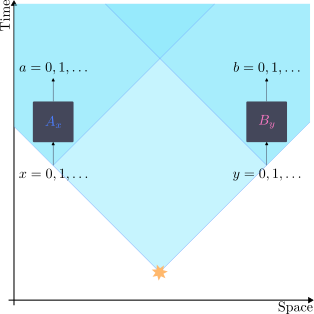
\includegraphics[width=0.7\textwidth]{chapters/overview/img/belltest.pdf}
	\end{center}
	\caption{Bell game. Alice and Bob are space-like separated. Alice freely chooses an input $x$ and obtain an output $a$. Bob has input $y$ and output $b$.}
	\label{fig:belltest}
\end{figure}



\section{Non-signalling correlations}

\textit{Non-signalling} correlations are correlations respecting a single assumption: the measurement choice of one party can not influence the outcome of the other party's measurement.
When Alice and Bob are space-like separated, this assumption is enforced by special relativity, i.e. no information can be transmitted faster-than-light.

Formally, non-signalling correlations are correlations for which the local marginals of a party are independent of the other party's measurements choice. 
Mathematically, such correlations satisfy
\begin{align}
	\sum_b p(ab|xy) = \sum_b p(ab|xy') = p(a|x), \quad &\forall\,a,x,y,y' \\
	\sum_a p(ab|xy) = \sum_a p(ab|x'y) = p(b|y), \quad &\forall\,b,x,x',y.
	\label{eq:non-signalling}
\end{align}


\section{Local and non-local correlations}

\textit{Local correlations} are fully characterised from the local system of Alice and Bob, i.e. they are not influenced by any external factor.
This type of correlation accounts for some hypothetical shared hidden information between the two parties.
Indeed, since Alice and Bob were in contact in the past, outcomes of their measurements can be influenced by some past factors, available locally to both parties' systems but possibly unobservable.
These past factors are \textit{local-hidden variables} with arbitrary value that we represent using $\lambda$.
Moreover, because these variables might not stay constant throughout the game, we denote $q(\lambda)$ the probability distribution governing their evolution. 
From here, we can formally defined local correlations as any correlation that can be decomposed as
\begin{equation}
	p(ab|xy) = \int_\lambda \mathrm{d}\lambda \, q(\lambda) p(a|x,\lambda) p(b|y,\lambda).
	\label{eq:local}
\end{equation}
One assumption we made in writing this decomposition is the \textit{freedom of choice} of both parties' measurements, as $x$ and $y$ are independent of $\lambda$.

Interestingly, any local correlation can be written as a convex sum of deterministic local strategies, $p_i(ab|xy)=p(a|x,i)p(b|y,i)$, for which the output only depends on the input, following
\begin{equation}
	p(ab|xy) = \sum_i c_i p_i(ab|xy)
	\label{eq:polytope}
\end{equation}
where $c_i\geq 0$ and $\sum_i c_i = 1$.
From the previous decomposition it follows that the convex sum of local strategies is also local. 
Geometrically, the set of local correlations is the convex hull of a finite number of deterministic strategies, which is a convex polytope, the local polytope.

\medbreak

\textit{Non-local} correlations are defined as any correlation that can not admit be written in the form of \refeq{local}.
Such correlations can thus not be explained by means of local-hidden variable. 
Note that this is the case for some non-signalling correlations as correlations satisfying \refeq{non-signalling} do not necessarily admit a decomposition of the form \refeq{local}.
Conversely, local correlations respect the non-signalling assumption.

For a review on non-locality refer to \cite{Brunner14}.

\section{Quantum correlations}

\textit{Quantum correlations} occur when Alice and Bob each share a part of a quantum system, $\rho_{AB}$, that they prepared when they were in contact.
Generally, this quantum state is a mixed state laying in the Hilbert space $\mathscr{H}^{AB} = \mathscr{H}^{A} \otimes \mathscr{H}^B$.
For measurements choice $x,y$, quantum correlations are given by Born's rule
\begin{equation}
	p(ab|xy) = \trr{\rho_{AB} M^a_x \otimes M^b_y} \quad \forall\,a,b,x,y
	\label{eq:Born}
\end{equation}
where $M^a_x$ is the \acrfull{povm} element of measurement $A_x$ associated with outcome $a$, and similarly for Bob with the \acrshort{povm} $M^b_y$ for measurement $B_y$ and outcome $b$.

\medbreak

Quantum correlations satisfy the non-signalling assumption, but are not necessarily local.
In order to obtain non-local quantum correlations, Alice and Bob must share an entangled state as the correlation produced by an entangled state
\begin{equation}
	\begin{split}
		p(ab|xy) &= \trr{\rho_{AB} \, M^a_x \otimes M^b_y} \\
				 &= \sum_i c_i\, \trr{(\rho^A_i \otimes \rho^B_i) (M^a_x \otimes M^b_y)} \\
				 &= \sum_i c_i\, \trr{\rho^A_i M^a_x \otimes \rho^B_i M^b_y} \\
				 &= \sum_i c_i\, p(a|x,i)\, p(b|y,i)
	\end{split}
\end{equation}
is of the form \refeq{polytope} and thus local.
Entanglement can thus be detected from the presence of non-local correlations, given that the non-signalling assumption is enforced.

\section{Bell inequalities}

In his 1964 paper, John Bell proposed a theorem which bounds the correlation that can be obtain by local-hidden variables theories~\cite{Bell1964}.
These bounds are know as \textit{Bell inequalities}.
Facets of the local polytopes are examples of such Bell inequalities.
When a Bell inequality is not satisfied by some correlation, we observe a \textit{Bell violation}.
Consequently, violating a Bell inequality proves the presence of non-locality and, therefore, of entanglement.

\medbreak

The most general expression of a Bell inequality $\mathcal{I}$ on some correlation $\mathbf{P}$ is
\begin{equation}
	\mathcal{I}(\mathbf{P}) = \sum_{a,b,x,y}c_{abxy} p(ab|xy) \leq \beta_L
	\label{eq:bell_inequality}
\end{equation}
where $\beta_L$ is the \textit{local bound}, i.e. the maximum value such that $\mathbf{P}$ is compatible with local realism.

\section{CHSH inequality}

\acrfull{chsh}, in a effort to experimentally test Bell's theorem, proposed a more specific version of Bell's game and inequality~\cite{Clauser1969}.
The game, today known as the \textit{\acrshort{chsh} game}, limits Alice and Bob to two dichotomic measurements, $A_0,A_1$ for Alice and $B_0,B_1$ Bob, with outcomes $a,b\in\{\pm 1\}$. 
A well-suited Bell inequality for this game is the \acrshort{chsh} inequality 
\begin{equation}
	S = \left | \mean{A_0 B_0} + \mean{A_0 B_1} + \mean{A_1 B_0} - \mean{A_1 B_1}  \right | \leq 2
	\label{eq:CHSH}
\end{equation}
where $S$ is the \textit{CHSH score}, and $\mean{A_x B_y} = \sum_{a,b} ab\,p(ab|xy)$ expresses a \textit{correlator} -- quantifying how correlated are the outcomes of two measurements.
Note that correlators of a quantum state $\rho_{AB}$ are defined using Born's rule $\mean{A_x,B_y} = \trr{\rho_{AB} A_X \otimes B_y}$.
It is convenient to define the \acrshort{chsh} operator, a Bell operator,
\begin{equation}
	\mathcal{B}_{\mathrm{CHSH}} = A_0 \otimes \left( B_0 + B_1 \right) + A_1 \otimes \left( B_0 - B_1 \right)
	\label{eq:CHSH_operator}
\end{equation}
from which the \acrshort{chsh} score can be obtain using $S = \left| \trr{\mathcal{B}_\mathrm{CHSH}\, \rho_{AB} } \right|$.

\medbreak

This inequality can be used to prove the non-local nature of quantum mechanics. 
Consider the $\ket{\psi^-}$ Bell state, also known as the \textit{singlet} state, shared between Alice and Bob, and the measurements
\begin{equation}
	\begin{split}
		A_0 = \sigma_z, \quad & \quad A_1 = \sigma_x \\
		B_0 = \frac{\sigma_z+\sigma_x}{2}, \quad &\quad B_1 = \frac{\sigma_z - \sigma_x}{2}.
		\label{eq:CHSH_measurement}
	\end{split}
\end{equation}
Computing the \acrshort{chsh} score from these resources yield $S=2\sqrt{2}$ which violates the inequality.
It can also be proven that $2\sqrt{2}$ is the maximum \acrshort{chsh} violation achievable using quantum resources~\cite{Tsirelson1980}.

\chapter{Quantum information}

Quantum entanglement and quantum non-locality gave birth to the field of quantum information and led to the second quantum revolution.
Indeed, if quantum mechanics revolutionized technology by using quantum proprieties to process classical information, mostly thanks to the transistor, there is now a shit to use quantum objects as a direct carrier of information.
Quantum information already have numerous technological application, from quantum computing to quantum cryptography, quantum simulation or quantum sensing to name a few.
For an introduction to quantum information see \cite{Nielsen2012}.

\section{Device-independent quantum information processing}

Quantum information processing rely heavily on quantum non-locality and consequently on quantum entanglement.
It is then necessary to certify that a proposed implementation carries out some form of entanglement.
A possible approach is to use quantum state tomography, which allows to reconstruct the density matrix of a quantum state~\cite{MauroDAriano2003}.
Another possibility is perform entanglement witnesses, measuring a target quantum state against specific operators, see e.g. \cite{Bru2002}.
On the downside, these two methods require precisely calibrated measurement devices, which is a major experimental challenge.

To circumvent this problem, one can use a \texit{device-independent} approach, in which all the quantum devices used, both for the implementation and the entanglement certification, are considered as black-boxes, i.e. no assumption are made on their inner working.
As we saw in the previous chapter, a Bell inequality violation certifies the non-local nature of a tested correlation, and thus assert the presence of entanglement.
Hence, a Bell violation is a device-independent certification of entanglement, as it does not require any assumption on how the tested correlation was obtain, i.e. the inputs $x,y$ and outputs $a,b$ are treated as pure mathematical object with no specific physical nature.
Notice however, that such certification still requires some assumption on the Bell test itself, as free-will and the spatial separation of the parties are required.

\medbreak

The device-independent approach goes beyond the simple certification of entanglement and is at the core of complex quantum information technologies.
\acrfull{diqkd} is possibly one of the most characteristic of such technologies~\cite{Pironio2009,Nadlinger2022}.
\acrshort{diqkd} allow two parties to share a secret key whose secrecy is guarantee by the law of physics and without making assumptions on the quantum devices used to produce that key.
The simplest device-independent protocol is self-testing, the device-independent characterisation of quantum state and measurements~\cite{Supic2019}.
Another great example of device-independent technology is blind distributed quantum computing, where a client with a small quantum apparatus can distribute a quantum computing task to a distant server and certify the privacy of the computation as well as its integrity~\cite{Fitzsimons2017}.
Other notable device-independent protocols is the device-independent generation of random number of quantum origin~\cite{Liu2018}.

\section{Self-testing}

Introduced by Mayers and Yao, self-testing is the cornerstone of device-independent protocols~\cite{Mayers2004}.
Its use case apply when a classical client, with access to multiple black-boxes would like to certify that these boxes performed specific measurements on a specific shared quantum state producing non-local correlations.
Each boxes has some inputs the client can chose freely, and some outputs they can record, that together form some correlations, similarly to a Bell game.
Self-testing protocols tests these correlations against a Bell inequality crafted to certify the presence of a specific state and measurements.
More precisely, the maximum violation of some Bell inequality can only be achieve by a particular family of correlations, yield only by a specific state and measurements.
The first self-testing protocol use the \acrshort{chsh} inequality to certify the presence of a maximally entangled two-qubit state~\cite{Mayers2004}. 
New protocols then extended self-testing, notably to all pure bipartite entangled two-qubit states~\cite{Yang2013,Bamps2015}, and even to any pure bipartite entangled state~\cite{Coladangelo2017}. 
For a in-depth review on self-testing, see \cite{Supic2019}.

\medbreak

This device-independent approach is crucial when the black-box devices, untrustworthy, are used to generate the state and perform the measurement for a quantum information processing task.
Hence, self-testing was proposed has a method to perform device-independent quantum key distribution~\cite{Mayers2004}, verifiable blind quantum computing~\cite{Gheorghiu2015,Gheorghiu2017}, certify part or the entirety of a quantum circuit~\cite{Magniez2006,Sekatski2018}, or certify a quantum network link~\cite{Bancal2021}.
However, it worth noting that for some device-independent protocols, correlations can be directly and more efficiently used to prove the correct inner working of the black-boxes, without resorting to self-testing.

\medbreak

Originally, self-testing aims at certifying exactly a given state and measurements thanks to the maximum violation of a Bell inequality, only achievable by specific correlations~\cite{Mayers2004}
Experimentally, this is challenging as noises and losses will introduce bias and because the exact correlations of a system can not be perfectly obtained as it requires an infinite sample size of game rounds.
To circumvent these issues, \textit{robust self-testing} was introduce as a mean to approximate a self-test certificate~\cite{Kaniewski2016}
A robust self-test guarantees that if a sufficiently high Bell violation is observed, the state and measurements are \textit{close} to the ones we would like to certify.
Alternatively, from a high enough violation, one can expect to \textit{extract} a state close to the target one.
Robust self-testing protocols were developed to decrease the requirement on the Bell violation while maintaining a certain closeness to the state to certify~\cite{Bancal2015,Kaniewski2016,Kaniewski2017,Valcarce2022}.
